% tikzpic.tex
\documentclass[crop,tikz]{standalone}% 'crop' is the default for v1.0, before it was 'preview'

\usetikzlibrary{arrows,decorations.pathmorphing,decorations.pathreplacing,backgrounds,positioning,fit,matrix}
\usetikzlibrary{shapes,calc,patterns,arrows.meta}
\tikzset{
	vert/.style={circle,inner sep=1.5,fill=white,draw,minimum size=.3cm},
	edge/.style={color=black, thick},
	diredge/.style={->,>={Stealth[width=8pt,length=8pt]},color=black, thick},
	timelabel/.style={fill=white,font=\footnotesize, text centered},
	wave/.style={decorate,decoration={coil,aspect=0}},
	dirwave/.style={->, >={Stealth[width=8pt,length=8pt]},decorate,decoration={coil,aspect=0}},
	diredge2/.style={->,>={Stealth[width=8pt,length=8pt]}}
}
\begin{document}


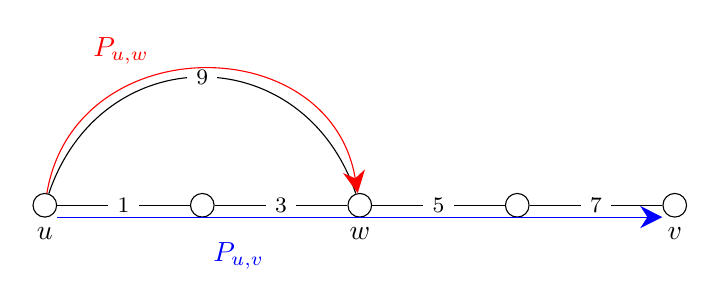
\begin{tikzpicture}[xscale=2]
	%%%S_uv
	\node[vert,label=below:$u$] (v1) at (1,0) {};
	\node[vert] (v2) at (2,0) {};
	\node[vert,label=below:$w$] (v3) at (3,0) {};
	\node[vert] (v4) at (4,0) {};
	\node[vert,label=below:$v$] (v5) at (5,0) {};
	\draw (v1) -- node[timelabel] {$1$} (v2) -- node[timelabel] {$3$}  (v3) -- node[timelabel] {$5$} (v4) -- node[timelabel] {$7$} (v5);
	\draw (v1) to [out=80,in=100,distance=2cm] node[timelabel] {$9$} (v3);
	
	\draw[transform canvas={yshift=-1.5mm}, blue]
	(v1) edge[diredge2]  node[pos=0.3,yshift=-2,label=below:$P_{u,v}$] {} (v5) ;
	
	\draw[red]
	(v1) edge[diredge2] [out=85,in=95,distance=2.1cm] node[pos=0.3,yshift=2,label=above:$P_{u,w}$] {} (v3) ;
\end{tikzpicture}

\end{document}